%==============================================================================
\section{Resultados}\label{resultados}
%==============================================================================
A partir da implementação do software foi possível construir uma ferramenta de auxilio a execução de processos. O software apesar de simples possui uma estrutura robusta, possibilitada pela componentização que a linguagem Java oferece, podendo ter suas funcionalidades aumentadas ao longo do tempo.

Na figura \ref{figura:selecaoarquivo} é apresentado a estrutura no qual o usuário seleciona o arquivo SPEM. O arquivo pode ser gerado a partir de um processo modelado na ferramenta EPF Composer.
\begin{figure}[!htb]
	\caption{Seleção Arquivo}
	\label{figura:selecaoarquivo}
	\centering
	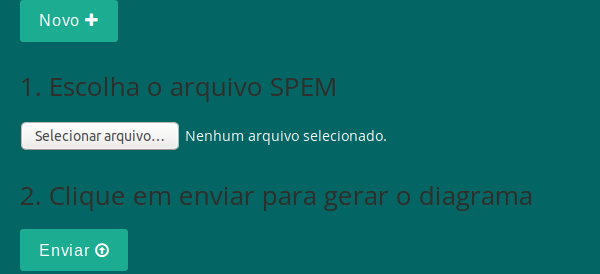
\includegraphics[width=1\textwidth]{img/ferramenta_selecao_arquivo.png}
\end{figure}

Após o arquivo ser selecionado o usuário necessita apenas clicar no botão enviar. Com o arquivo no formato SPEM enviado para o servidor, a ferramenta vai gerar um diagrama como mostrado na figura \ref{figura:diagramagerado}.

\begin{figure}[!htb]
	\caption{Diagrama Gerado}
	\label{figura:diagramagerado}
	\centering
	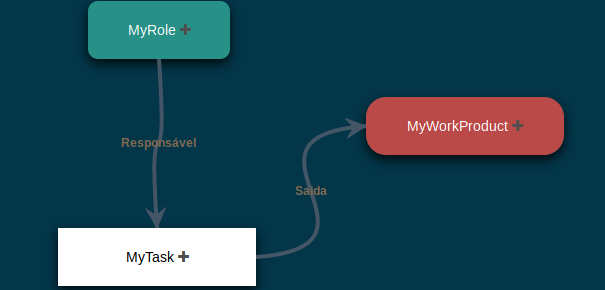
\includegraphics[width=1\textwidth]{img/ferramenta_diagrama_gerado.png}
\end{figure}

Este diagrama pode ser utilizado para controlar o fluxo das atividades, sendo possível finalizar cada atividade completada. Além disso é possível anexar arquivos a cada artefato da atividade, podendo ser posteriormente acessado novamente.